\begin{figure}[!ht]
	\centering
	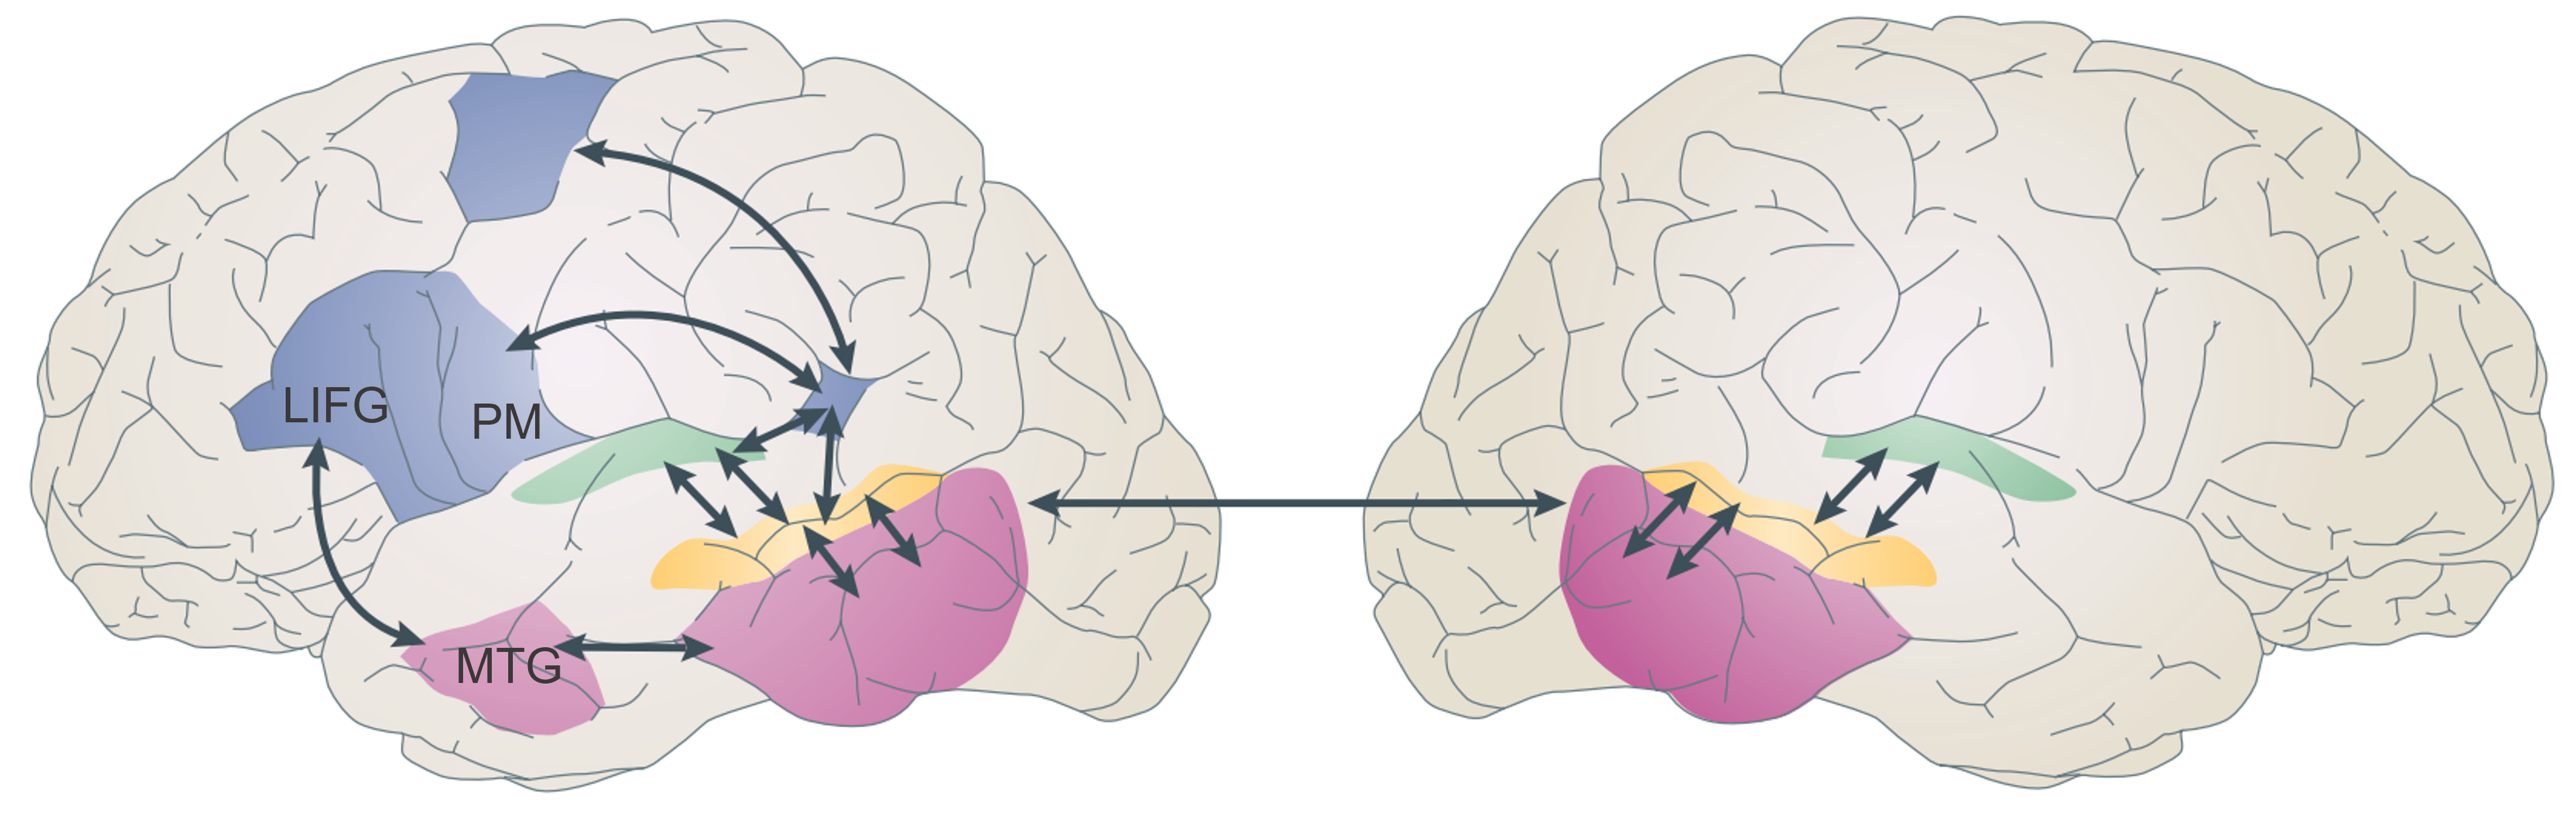
\includegraphics[width=.9\textwidth, clip=true]{./Chapters/01_Introduction/Images_MM/Language_network}
	\caption{Brain structures involved in language comprehension and production. Colors indicate different functional roles: pink = lexico-semantic interface, yellow = phonological network, green = spectrotemporal analysis of speech sounds, blue = articulatory network. LIFG = left inferior frontal gyrus, PM = premotor cortex, MTG = middle temporal gyrus. Figure adapted from \citet{hickok2007}}
    \vspace*{-10pt}
	\label{fig:language}
\end{figure}